\chapter{Estado de Arte}
\label{sec:estado-arte}

Neste capítulo será feita a comparação de algumas plataformas existentes para recolha de dados com recurso a estratégias de inbound marketing. Será também feito um resumo das funcionalidades do \acrshort{tcg}, que apesar de já estar no mercado, será integrado neste projeto. Tendo em conta que a plataforma a desenvolver irá utilizar as funcionalidades para criação de formações do \acrshort{tcg} e que a equipa do \acrlong{tcg} já fez o estudo de mercado antes do desenvolvimento do mesmo, e continua a fazer todos os dias, a análise de plataformas focadas em criação de formações não será feita neste documento. Uma análise mais detalhadas de todas as plataformas estudadas encontra-se no Anexo \ref{a:ea}.

A recolha de informação nos dias de hoje tem um grande impacto na forma como os negócios são feitos, principalmente na internet.

Como referido no capítulo anterior, o objectivo deste estágio incide na criação de uma plataforma de inbound marketing que tem como principais objectivos conseguir criar e partilhar campanhas, e através da analise e segmentação dos dados recolhidos, optimizar novas outras campanhas. Neste sentido serão analisadas algumas das soluções existentes que, apesar de algumas terem um propósito distinto, podem ser utilizadas em estratégias de inbound marketing e partilham funcionalidades semelhantes com o que vai ser desenvolvido. 

A recolha de informação nos dias de hoje tem um grande impacto na forma como os negócios são feitos, principalmente na internet. Seguindo uma das estratégias de inbound marketing, o método de recolha de dados será através de campanhas que podem ser concursos, questionários de personalidade e/ou formações online e por isso mesmo, algumas características associadas à experiência do utilizador, como por exemplo a personalização dos mesmos, serão também analisadas.

%Rever o que está para baixo

As plataformas \textit{SurveyMonkey}\cite{surveymonkey}, \textit{Typeform}\cite{typeform}, \textit{Google Forms}\cite{googleform} são plataformas de criação de formulários, mas apesar de servirem um propósito distinto ao da plataforma a desenvolver, partilham funcionalidades semelhantes com as que vão ser desenvolvidas e por isso mesmo serão analisadas nesse sentido. Será também exposto o funcionamento do \acrshort{tcg} para um melhor entendimento de como podem ser implementadas as funcionalidades e a \acrshort{api} do lado da plataforma a desenvolver. A integração do \acrshort{tcg} neste projeto, foi uma escolha da empresa (i. e. cliente), e por isso não serão analisadas plataformas concorrentes do \acrshort{tcg} na medida em que esse trabalho é feito pela equipa do \acrshort{tcg} e apenas serão feitas as mudanças necessárias no mesmo para o desenvolvimento da \acrshort{api} de comunicação. Por último serão analisadas as plataformas \textit{involve.me}\cite{involve}, \textit{Survey Anyplace}\cite{surveyA} e \textit{Interact}\cite{interact} que são alguns das serviços que podem concorrer directamente com o 10.quest (i. e. plataforma a desenvolver).

Após a apresentação destas ferramentas será feita uma análise das vantagens e desvantagens de cada uma, assim como a comparação de funcionalidades.

\section{Análise de plataformas de criação de formulários (concorrentes indiretos)}
\label{formulários}

Nesta secção serão analisadas e comparadas três das ferramentas líderes na criação de formulários online. Estas ferramentas são o \textit{SurveyMonkey}, \textit{Typeform} e \textit{Google Form} e apesar de serem plataformas que não concorrem com o 10.quest (i. e. o 10.quest não será desenviolvido para criar formulários) e terem um propósito bastante distinto, partilham funcionalidades que podem ser semelhantes com a plataforma que vai ser desenvolvida. Dito isto é importante perceber quais são estas funcionalidades e tentar perceber como as podemos aproveitar ou melhorar.


O SurveyMonkey é uma plataforma \acrfull{saas} de criação de formulários e questionários online para estudo de mercado, análise de competidores, \textit{feedback} de clientes e colaboradores, entre outros. Permite recolher informações do público alvo através de formulários e questionários, e personalizar, segmentar e visualizar esta informação.
%As várias funcionalidades do SurveyMonkey foram desenhadas para ajudar os utilizadores a criar diferentes tipos de formulários e questionários, e recolher os resultados. Estes dados são depois analisados e reportados através de funcionalidades próprias do SurveyMonkey. Estes dados podem ainda ser exportados para satisfazer outras necessidades. 
Os principais aspectos e funcionalidades principais do SurveyMonkey são:
\begin{itemize}
	\item Login e registo através de APIs externas;
	\item Plano gratuito com funcionalidades limitadas. Planos pagos com acesso a mais funcionalidades;
	\item Criar formulários e questionátios;
	\item Formulários e questionários modelo, organizados por categorias;
	\item Criar vários tipos de perguntas (i. e. pergunta simples, escolha múltipla, avaliação com estrelas, caixa de seleção, upload de arquivo, data e hora etc..);
	\item Perguntas modelo, organizadas por categoria;
	\item Anexar imagens e vídeos a perguntas e respostas;
	\item Personalizar a aparência dos formulários e questionários;
	\item Fluxo lógico de perguntas;
	\item Pré-visualizar formulários e questionários antes de publicar;
	\item Vários métodos de partilha de formulários e questionários (i. e. através de um link, por email, rede social etc...);
	\item Aceita pagamentos;
	\item Suporte dedicado;
	\item Colaboração;
	\item \textit{Branding} personalizado;
	\item Análise de dados:
		\subitem Percentagem de respostas por pergunta;
		\subitem Possível filtrar dados por pergunta;
		\subitem Exportar dados.
		
\end{itemize}

O \textit{Google Form} é uma aplicação de administração de inquéritos que está incluída no Google Drive office juntamente com o \textit{Google Docs}\cite{gdocs}, \textit{Google Sheets} e \textit{Google Slides}\cite{gslides}. Esta ferramenta permite recolher informações do público alvo através de formulários e inquéritos personalizados e automaticamente exportar os dados para uma \textit{google sheet}. Os principais aspectos e funcionalidades principais do \textit{Google Form}  são:
\begin{itemize}
	\item Gratuito
	\item Vários formulários modelo.
	\item Criar vários tipos de perguntas (i. e. pergunta simples, escolha múltipla, escala linear, carregamento de ficheiro, \textit{dropdown} etc..); 
	\item Anexar imagens e vídeos a perguntas e respostas;
	\item Personalizar a aparência dos fomulários; 
	\item Pré-visualizar formulários e questionários antes de publicar;
	\item Partilhar formulário através de link, ou embebido numa página web;
	\item Colaboração;
\end{itemize}


O Typeform é uma plataforma \acrshort{saas} de criação de formulários online. É uma empresa que afirma resolver o problema dos formulários e inquéritos aborrecidos e tem também como proposta de valor o facto de conseguir criar formulários e inquéritos sem ter que programar uma única linha de código. Esta plataforma permite recolher informações do público alvo através de formulários e inquéritos personalizados, podendo no final visualizar estes dados. 
Os principais aspectos e funcionalidades principais do Typeform são:
\begin{itemize}
	\item Login e registo através da API do Google;
	\item Plano gratuito com funcionalidades limitadas. Planos pagos com acesso a mais funcionalidades;
	\item Criar vários tipos de formulários (i. e. formulários, questionários, convites etc...);
	\item Vários formulários modelo.
	\item Criar vários tipos de perguntas (i. e. pergunta simples, escolha múltipla, avaliação, carregamento de ficheiro, \textit{dropdown} etc..); 
	\item Anexar imagens e vídeos a perguntas e respostas;
	\item Personalizar a aparência dos fomulários; 
	\item Fluxo lógico de perguntas; 
	\item Pré-visualizar formulários e questionários antes de publicar;
	\item Partilhar formulários através de um \textit{link}, ou pelas redes sociais;
	\item Aceita pagamentos;
	\item Integração com sistemas externos de geração de \textit{leads}, CRM e automação de marketing, análise e relatórios entre outros;
	\item Suporte dedicado;
	\item Colaboração;
	\item Subdomain costumizado;
	\item Remover \textit{branding}
	\item Análise de dados:
		\subitem Percentagem de respostas por pergunta;
		\subitem Taxa de conclusão dos formulários.
	
\end{itemize}


Como foi referido na análise, presente no anexo \ref{a:ea}, em todas as plataformas/ferramentas é necessário criar uma conta para aceder a todas as funcionalidades e em todas as plataformas analisadas é possível criar conta e iniciar sessão através de sistemas externos (\acrshort{api}). O Projeto a desenvolver segue um modelo \gls{b2b} e por isso mesmo não é de grande importância implementar esse tipo de funcionalidades.

A plataforma da \textit{Google} fornece, no plano gratuito, todas as funcionalidades, ao contrário do \textit{SurveyMonkey} e do \textit{Typeform}, que para se ter acesso a todas as funcionalidades, ou pacotes de funcionalidades, terá de ser paga uma subscrição. Na plataforma 10.Quest será também necessário pagar uma subscrição anual para aceder a todas as funcionalidades, contudo tem um periodo experimental de 30 dias (i. e. gratuitamente), a partir do dia de inscrição.

Todas as plataformas permitem a criação de formulários do zero, e a plataforma da 10.digital não é exceção, relativamente às campanhas. Tal como foi definido na estratégia de negócio, os conteúdos que serão lançados nas campanhas, não serão da autoridade da 10.digital, a menos que estejam incluídos em algum projeto relacionado. Dito isto facilmente se decidiu que a plataforma a desenvolver terá, tal como todas as outras ferramentas analisadas, a funcionalidade de poder adicionar conteúdo previamente feito de forma rápida (i. e. importar um ficheiro \textit{CSV} com todo o conteúdo estruturado). 


Tal como foi referido no capítulo \ref{sec:introducao}, secção \ref{subsec:contexto}, o inbound é uma estratégia de marketing que se foca em criar razões para atrair o público alvo, ou por outras palavras, fazer com que o público alvo procure a empresa. Para isto é necessária a criação de conteúdo interessante, útil, relevante etc... Para manter esta procura por parte dos clientes é necessário haver valor ao longo da jornada e idealmente proporcionar uma boa experiência ao utilizador. Nesta medida a personalização das campanhas é muito importante tanto a nível de conteúdo, como estético e funcional para que o utilizador se sinta valorizado. Para tornar isto possível, tal como o \textit{SurveyMonkey}, \textit{Typeform} e \textit{Google Form}, a plataforma a desenvolver incluirá funcionalidades que lhe permitirão personalizar a \textit{interface} das campanhas para melhorar a experiência do utilizador final. 

Como é visível na análise expressa no anexo\ref{a:ea} o \textit{SurveyMonkey} e o \textit{Typeform} integram a funcionalidade de criação de um fluxo lógico. Contudo esta funcionalidade será abordada mais à frente nesta dissertação, com o intuito de fazer uma análise  mais aprofundada e comparativa com as plataformas directamente concorrentes.

Antes de enviar/partilhar um formulário é sempre importante pré-visualizar e testar. Neste aspecto a plataforma a desenvolver não é diferente. Será possível pré-visualizar as campanhas para verificar e validar as mesmos. 

Por último temos o tratamento e visualização de dados que é um suporte fundamental ao marketing digital. A plataforma a desenvolver, a par com todas as restantes plataformas analisadas, não é um \textit{software} dedicado a esse fim, na medida que terá limitações (i. e. apenas implementa um conjunto de funcionalidades principais de tratamento e visualização de dados para satisfazer as necessidades do utilizador. Funcionalidades como a remoção de \textit{outliers}, calculo da previsão dos dados etc..., que envolve uma tratamento mais cuidado e por vezes não linear, não são implementadas), contudo, terá as funcionalidades necessárias (i. e. percentagem ou funil de participação em campanhas, utilizadores abrangidos, lista de leads, lista de resultados e tags mais frequentes (têndencias), percentagem de respostas correctas por tag, gráfico de eventos, entre outros) para satisfazer as necessidades do utilizador. A plataforma \textit{SurveyMonkey}, neste aspecto, foi a única ferramenta que apresentou funcionalidades para além da análise básica conseguindo, de forma elementar, segmentar e comparar resultados, em contraste com o \textit{Typeform} e do \textit{Google Form} que apenas apresentam os resultados globais e por pergunta.

\section{\acrfull{tcg}}
\label{sec:TCGM}

O \acrlong{tcg} é um \acrshort{saas} presente atualmente no mercado, desenvolvido pela equipa da 10.digital, que tem como principal objectivo transmitir conhecimento através de uma técnica de aprendizagem baseada em tentativa e erro.


O \acrshort{tcg} nasceu de uma forte convicção de que perder apenas 2 minutos por dia numa formação com uma abordagem tentativa e erro é uma ótima forma de aprender, poupando tempo e dinheiro às empresas. Inicialmente muito focado em formação interna, a equipa do \acrshort{tcg} foi-se apercebendo que existem muitos outros problemas (e. g. Consolidação de procedimentos, \textit{Onboarding} de novos colaboradores, Divulgação da cultura da empresa, Divulgação de informações técnicas a parceiros/clientes ...) para o qual a plataforma tem solução (e. g. Assimilação da cultura de empresa e do espírito das marcas, Simplificação do processo de acolhimento, Redução de custos em reuniões periódicas, Facilidade em divulgar aspectos técnicos, que de outra, forma demorariam mais tempo ...).\cite{tcginfo}. 

As principais funcionalidades do  \acrshort{tcg}  são as seguintes:


\begin{itemize}
	\item[--] Criação de formações 
	\item[--] Tutoriais para as funcionalidades chave
	\item[--] Algoritmo de gestão automática (i. e. sistema identifica as perguntas mais difíceis baseado nos resultados do utilizador final. As perguntas mais difíceis saem com mais frequência e perguntas erradas saem no dia seguinte)
	\item[--] \textit{Feedback }dos utilizadores em cada pergunta
	\item[--] \textit{Gamification}
	\item[--] Análise detalhada dos resultados
	\item[--] Compatível com dispositivos móveis
\end{itemize}

\section{Análise de concorrentes directos}

Um dos objetivos do projeto é permitir aos utilizadores da plataforma a criação de questionários que, baseando-se nas respostas do utilizador final, apresenta um resultado  segmentado no fim do mesmo, tal como referido no Capítulo \ref{subsec:objetivos}.

O Akinator\cite{akinator} e o high5test\cite{5} são dois bons exemplos de aplicações que através de um questionário, e baseado nas respostas do utilizador final, apresenta um resultado segmentado. Estas duas aplicações são bastante poderosas e utilizam algoritmos de decisão que os permitem tirar este tipo de conclusões. Nesta medida alguns algoritmos como o CART\cite{cart}, ID3\cite{id3}\cite{id3_2}\cite{cart} e C4.5\cite{cart}\cite{c4.5} foram brevemente estudados com intuito de avaliar a viabilidade de serem aplicados na conceção desta funcionalidade do projeto. Este tipo de algoritmos, não só são complexos como são algoritmos que necessitam de dados de treino. Tal como referido no Capítulo \ref{subsec:objetivos}, um dos requisitos definidos pelo cliente é que a criação destes questionário seja intuitiva e exequível por qualquer pessoa mesmo que esta não tenha qualquer conhecimento em programação. Isto agregado ao facto de que, em qualquer momento da criação dos questionário, não haverá dados de treino, a aplicação deste tipo de algoritmos não é viável.

Dito isto foram discutidas outras abordagens e determinou-se que uma possível boa solução, que vai de encontro ao conceito da funcionalidade, passa pela criação de um sistema recomendação.
Nesta abordagem são atribuídos pesos a cada pergunta e tags às respectivas respostas. O peso determina o impacto que cada pergunta tem no calculo do resultado, e consoante a resposta do utilizador, o sistema vai organizando os resultados num ranking de recomendação baseado na pontuação da pergunta e na correspondência entre as tags associadas às respostas e as tags associadas aos resultados. Este algoritmo de recomendação será mais detalhados nas secções \ref{d:quests} e \ref{sec:val_alg}.

Uma aplicação deste tipo de questionário será, por exemplo: "Calcule o lugar ideal de para viajar nas suas férias". Atualmente, num formato semelhante (i. e. em formato \textit{quiz}) já existem alguns \textit{Websites} (e. g. Chase for Adventure\cite{chaseforadventure}, travelpicker\cite{travelpicker}, Insight Vacations\cite{insightvacations} e Driftwood Journals\cite{driftwoodjournals}) que satisfazem, de forma simplista, esta necessidade em específico. Apesar de simples são exemplos que se conseguirião replicar com a plataforma a desenvolver e que está alinhado com a visão da plataforma. Neste sentido foram analisadas plataformas mais poderosas, que se focam na construção de leads, e que conseguem um resultado semelhante.


\subsection{involve.me}
\label{involvemeM}

%Não aceita multiplos resultados por resposta
%não cria perfis de utilizador
%multichannel supporte
%landiung page

"\textit{involve.me is a next-generation user engagement \& customer experience platform with a focus on digital marketers \& e-commerce.}"\cite{involve}. O involve.me é uma plataforma moderna que ajuda empresas a criar interações personalizadas ao longo da jornada dos clientes, aumentando a audiência e recolhendo mais e melhores dados. Esta plataforma foca-se também na recolha e análise destes dados/informações sobre os utilizadores finais.


\subsection{Survey Anyplace}
\label{surveyanyplaceM}


%nao avisa que está live o questionário
%feature de ajuda no canto inferior direito -  multi channel


O Survey Anyplace é uma plataforma online com foco na criação de \textit{surveys} e questionários interativos. O Survey Anyplace afirma proporcionar uma boa experiência para o utilizador facultando-lhe elementos interativos e funcionalidades de personalização. Esta plataforma permite também a análise dos dados recolhidos através dos questionários publicados.


\subsection{Interact}
\label{interactM}


O Interact é uma das grandes plataformas de criação de questionários e geração de \textit{leads}. Um dos principais focos da empresa, para além da geração de leads, é a segmentação da audiência. " Interact is a tool for creating online quizzes that generate leads, segment your audience, and drive traffic to your website. "\cite{interact}.



\subsection{easypromo}
\label{easypromoM}

\textit{Easypromos}\cite{f6} é uma plataforma para criação e gestão de campanhas, questionários, concursos, promoções etc.. A \textit{easypromos} afirma que a sua plataforma aumenta o número de seguidores das marcas, melhora a sua visibilidade, gera um maior número de \textit{leads} e ajuda na conversão dos mesmos para clientes.


\subsection{Discussão de funcionalidades}
\label{comparacao}

\subsubsection{Questionários}

Nas tabelas \ref{tab:comparacao1}, \ref{tab:comparacao2} e \ref{tab:comparacao3} encontra-se a comparação entre as plataformas analisadas no Anexo \ref{a:ea}, baseada numa lista de funcionalidades.

Como vimos na análise efetuada no Anexo \ref{a:ea}, em todas as plataformas/ferramentas é necessário criar uma conta para aceder a todas as funcionalidades, contudo apenas o \textit{involve.me} e p \textit{easypromos} fornecem um plano gratuito que dá acesso apenas a algumas funcionalidades. As restantes plataformas apenas disponibilizam um plano trial que fornece o acesso a um pacote de funcionalidades pago, durante 6 dias(\textit{Survey Anyplace}), 15 dias(\textit{Interact}) ou 30 dias (10.quest). No fim deste prazo, os utilizadores, para continuarem a usufruir das funcionalidades da plataforma terão de subscrever um plano/pacote de funcionalidades.

Todas as ferramentas analisadas disponibilizam uma série de templates excepto o 10.quest que não prevê a integração dessa funcionalidade num futuro próximo. Todas as ferramentas permitem a criação de questionários do zero e todas elas possuem ferramentas de personalização dos mesmos.

De entre todas as plataformas analisadas o 10.quest é a unica que permite importar conteúdo previamente feito com recurso a ficheiros externos (i.e. perguntas e respostas ou resultados através de um ficheiro CSV). É de notar que as questões importadas para a plataforma através desta funcionalidade, tendo em conta que esse processo é feito através de uma \textit{spreadsheet}, ficheiros de imagens ou vídeo terão de ser adicionados posteriormente.

Cada plataforma tem a seu método de criar um fluxo lógico ou sistema de pontuações para conseguir calcular o resultado segmentado de acordo com as respostas do utilizador final. O \textit{involve.me} desmonstrou ser a ferramenta mais fraca no que a esta funcionalidade diz respeito, visto que apenas se pode associar um resultado possível a uma resposta. O \textit{easypromos} implementa um sistema correlação com as resultados possívo. O utilizador cria uma série de resultados e atribui a cada um número (categoria), o resultado final será o resultado cuja sua categoria foi escolhida mais vezes. Uma desvantagem deste método é que não se consegue atribuir maior importância a uma determinada pergunta. O \textit{Survey Anyplace} e o 10.quest demonstram ser as plataformas com maior capacidade de implementar estas funcionalidades visto que ambos integram um sistema de pontuações e sistema de recomendação, respectivamente, sendo que o \textit{Survey Anyplace} consegue criar um fluxo lógico. O \textit{Interact} consegue associar resultados a respostas contudo todas as ligações valem o mesmo e por isso mesmo o cálculo do resultado final não é tão preciso.


Depois de terminado um questionário é necessário pré-visualizar o mesmo para verificar se tudo está de acordo com o idealizado e tal como em todas as plataformas analisadas, o 10.quest terá essa funcionalidade.

Para partilhar os questionários, o \textit{Survey Anyplace} fica um pouco atrás de todas as outras plataformas visto que não inclui a partilha dos questionários nas redes sociais, dentro da plataforma. Apesar disso o \textit{Survey Anyplace} gera um link para ser partilhado, tal como em todas as plataformas restantes, e possibilita a integração do questionário noutro \textit{website}. 
%Por decisão do cliente o 10.quest não permite ser embebido noutros \textit{websites}. 
Outra maneira de partilhar as campanhas será através de um link ou através das redes sociais. Desta forma é partilhada uma \textit{landing page} onde o utilizador final se inscreve/subscreve e de seguida recebe o link para a campanha por email. As únicas plataformas que implementam e automatizam este processo são o \textit{Interact} e o 10.quest.

Na secção de recolha e análise de dados a 10.quest destaca-se. A 10.quest é unica plataforma que apresenta estatísticas globais que satisfazem as necessidades do utilizador (i. e. que representam dados relevantes), na criação de perfis de personalidade. É também a única plataforma que tem capacidade de associar as tags das campanhas a utilizadores finais e assim criar perfis de personalidade conseguindo segmentar leads qualificadas. Estas tags são associadas às campanhas, e assim que um utilizador final se inscrever nas mesmas, a tag é automaticamente associada ao utilizador final.  À semelhaça da plataforma \textit{Interact} o 10.quest mostra o túnel de conversão na análise de dados e gera um gráfico temporal de eventos que ajuda a perceber as tendências e as taxas de conversão ao longo do tempo.

O desenvolvimento desta plataforma joga também um papel importante em conseguir atingir os objectivos anuais da empresa e neste sentido alguns dos requisitos definidos para o projecto (secção \ref{sec:requisitos}) vão de acordo com as necessidades da empresa. Outro factor que contribui para a decisão é a flexibilidade e possibilidade de integração com outros sistemas internos.

\subsubsection{Concursos}

As plataformas \textit{easypromos} e 10.quest são as únicas plataformas capazes de criar concursos. 
Apesar de todas as plataformas terem múltiplas funcionalidades para criar e personalizar divertos tipos de pergunta, à excepção da \textit{easypromos} e do 10.quest, as restantes plataformas não apresentam os resultados em forma de \textit{leaderboard}, nem fazem o cálculo e atribuição de prémio ao vencedor de forma automática.
Todas as restantes funcionalidades associadas aos concursos, são muito semelhantes, com as funcionalidades descritas em cima e no Anexo \ref{a:ea}. 

\subsubsection{Tabela de comparações}


\begin{figure}[ht!]
	\begin{center}
		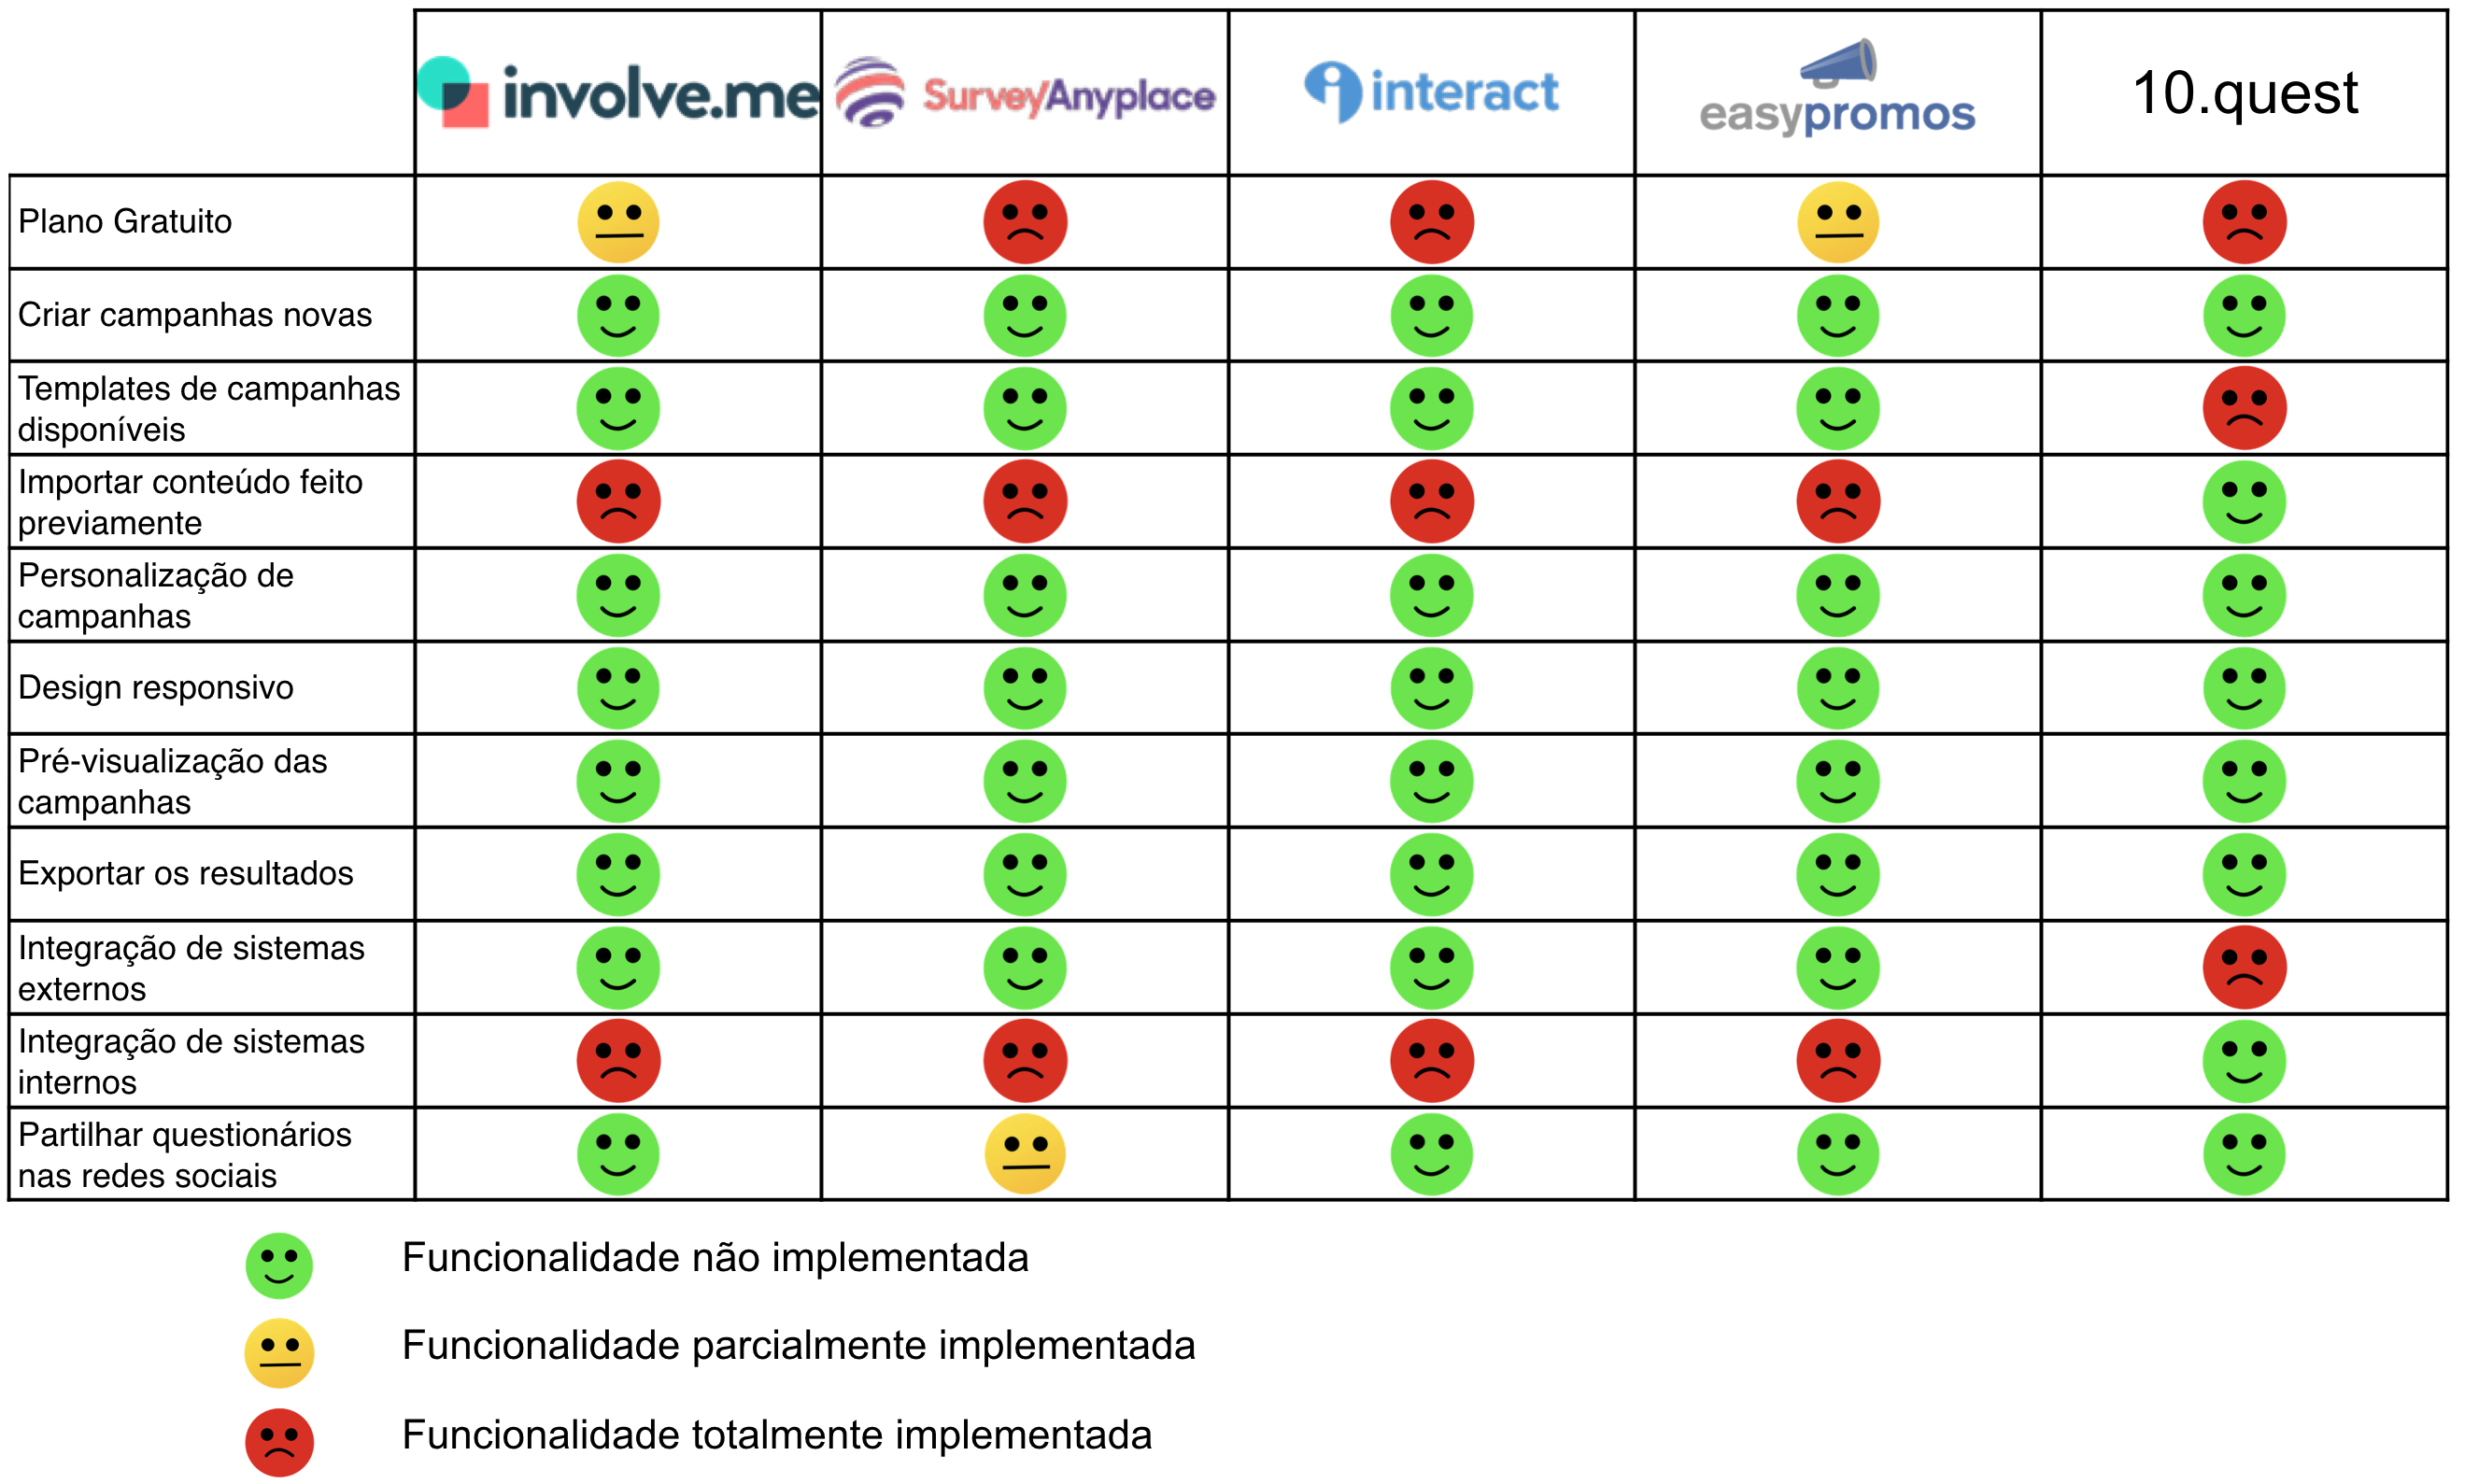
\includegraphics[width=1\textwidth]{img/ea/ea1}
		\captionof{table}[Tabela de comparação de funcionalidades]{Tabela de comparação de funcionalidades}
		\label{fig:ea-1}
	\end{center}
\end{figure}

\begin{figure}[ht!]
	\begin{center}
		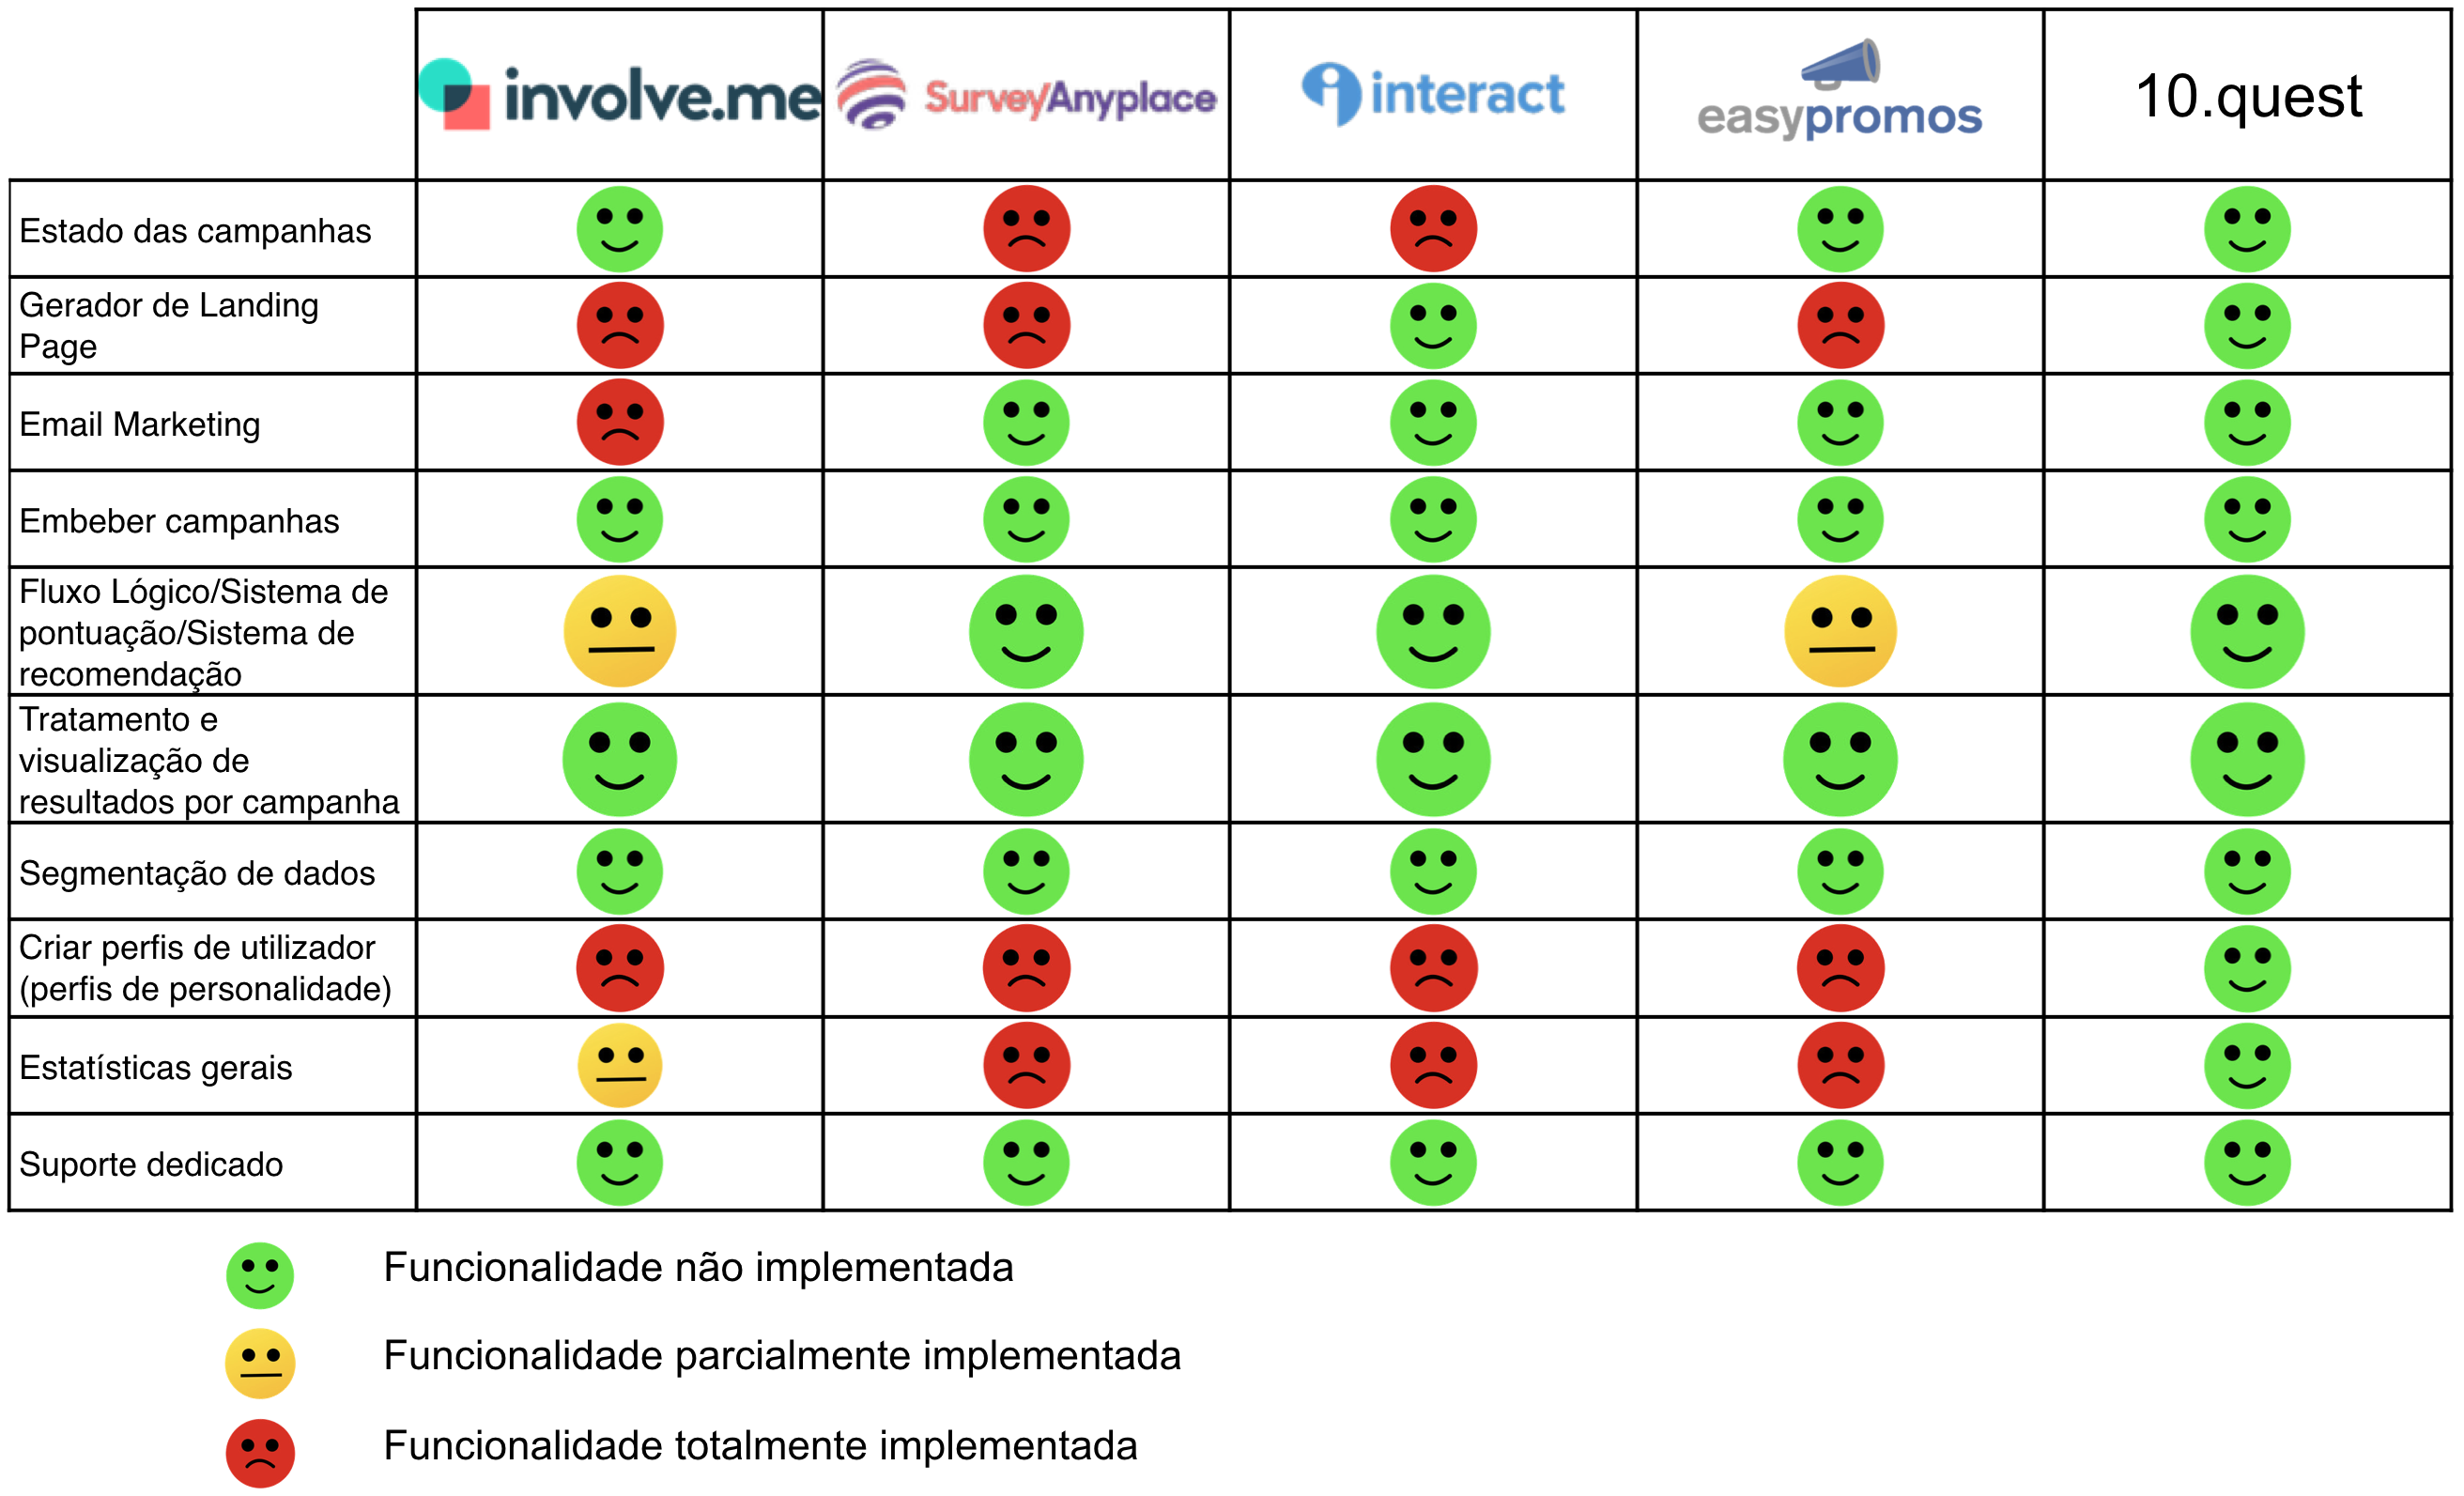
\includegraphics[width=1\textwidth]{img/ea/ea2}
		\captionof{table}[Tabela de comparação de funcionalidades (Continuação)]{Tabela de comparação de funcionalidades (Continuação)}
		\label{fig:ea-2}
	\end{center}
\end{figure}



\begin{comment}

\renewcommand{\arraystretch}{2}
\setlength\arrayrulewidth{1pt}
\begin{table}[!ht]  
	\begin{center}
		\begin{tabular}{|p{3cm}|p{0cm}|p{0cm}|p{0cm}|p{0cm}|p{0cm}|}
			\cline{2-6}
			\multicolumn{1}{c|}{} & \hspace{0.2cm}\begin{sideways}involve.me\end{sideways} & \hspace{0.4cm}\begin{sideways}Survey Anyplace\end{sideways} & \hspace{0.2cm}\begin{sideways}Interact\end{sideways}&
			\hspace{0.2cm}\begin{sideways}easypromos\end{sideways}& \hspace{0.2cm}\begin{sideways} 10.quest\end{sideways}\\ \hline
			
			
			Plano Gratuito & \cellcolor{yellow!80}   & \cellcolor{red!80}  & \cellcolor{red!80} & \cellcolor{yellow!80} & \cellcolor{yellow!80} \\ \hline
			
			Criar questionário novo & \cellcolor{green!80}  & \cellcolor{green!80}  & \cellcolor{green!80} & \cellcolor{green!80}  &\cellcolor{green!80} \\ \hline
			
			Templates de questionários disponíveis& \cellcolor{green!80}  & \cellcolor{green!80} & \cellcolor{green!80} & \cellcolor{green!80}  & \cellcolor{red!80}  \\ \hline		
			
			Importar conteúdo feito previamente & \cellcolor{red!80}   & \cellcolor{red!80}  & \cellcolor{red!80} & \cellcolor{red!80} & \cellcolor{green!80}  \\ \hline
			
			Personalização do questionário & \cellcolor{green!80}  & \cellcolor{green!80}  & \cellcolor{green!80} & \cellcolor{green!80} & \cellcolor{green!80} \\ \hline
			
			Criar perfis de utilizador & \cellcolor{red!80}   & \cellcolor{red!80}  & \cellcolor{red!80} & \cellcolor{red!80} & \cellcolor{green!80}  \\ \hline
			
		\end{tabular}
	\end{center}
	\hspace{1.2cm}	\textcolor{red}{$\blacksquare$} Funcionalidade não implementada
	
	\hspace{1.2cm}     \textcolor{yellow}{$\blacksquare$} Funcionalidade parcialmente implementada (i. e. não satisfaz totalmente as necessidades do utilizador)
	
	\hspace{1.2cm}     \textcolor{green}{$\blacksquare$} Funcionalidade totalmente implementada 
	\begin{center}
		\caption{Tabela de comparação de funcionalidades}
		\label{tab:comparacao1}
	\end{center}
\end{table}

\newpage

\renewcommand{\arraystretch}{2}
\setlength\arrayrulewidth{1pt}
\begin{table}[!ht]  
	\begin{center}
		\begin{tabular}{|p{3cm}|p{0cm}|p{0cm}|p{0cm}|p{0cm}|p{0cm}|}
			\cline{2-6}
			\multicolumn{1}{c|}{} & \hspace{0.2cm}\begin{sideways}involve.me\end{sideways} & \hspace{0.4cm}\begin{sideways}Survey Anyplace\end{sideways} & \hspace{0.2cm}\begin{sideways}Interact\end{sideways}&
			\hspace{0.2cm}\begin{sideways}easypromos\end{sideways}&
			\hspace{0.2cm}\begin{sideways} 10.quest\end{sideways}\\ \hline
			
			
			Pré-visualização dos questionários &\cellcolor{green!80}  & \cellcolor{green!80} & \cellcolor{green!80} & \cellcolor{green!80} & \cellcolor{green!80}  \\ \hline
			
			Exportar os resultados &\cellcolor{green!80}  & \cellcolor{green!80} & \cellcolor{green!80} & \cellcolor{green!80} & \cellcolor{green!80}  \\ \hline
			
			Integração de sistemas externos & \cellcolor{green!80}  & \cellcolor{green!80} & \cellcolor{green!80} & \cellcolor{green!80} & \cellcolor{red!80}  \\ \hline
			
			Partilhar questionários nas redes sociais &\cellcolor{green!80}  & \cellcolor{yellow!80} & \cellcolor{green!80} & \cellcolor{green!80} & \cellcolor{green!80}  \\ \hline
			
			
			Estado dos questionários &\cellcolor{green!80}  & \cellcolor{red!80} & \cellcolor{red!80} & \cellcolor{green!80}  & \cellcolor{green!80}  \\ \hline
			
			Gerador de \textit{Landing Page}  &\cellcolor{red!80}  & \cellcolor{red!80} & \cellcolor{green!80} & \cellcolor{red!80}  & \cellcolor{green!80}  \\ \hline
			
			Email Marketing &\cellcolor{red!80}  & \cellcolor{green!80} & \cellcolor{green!80} & \cellcolor{green!80} & \cellcolor{green!80}  \\ \hline
			
			Embeber questionários& \cellcolor{green!80}  & \cellcolor{green!80}  & \cellcolor{green!80} & \cellcolor{green!80} & \cellcolor{green!80}  \\ \hline
			
			Fluxo Lógico/Sistema de pontuação &\cellcolor{yellow!80}  & \cellcolor{green!80} & \cellcolor{green!80} & \cellcolor{yellow!80} & \cellcolor{green!80}  \\ \hline
			
			
			
		\end{tabular}
	\end{center}
	\hspace{1.2cm}	\textcolor{red}{$\blacksquare$} Funcionalidade não implementada
	
	\hspace{1.2cm}     \textcolor{yellow}{$\blacksquare$} Funcionalidade parcialmente implementada
	
	\hspace{1.2cm}     \textcolor{green}{$\blacksquare$} Funcionalidade totalmente implementada 
	\begin{center}
		\caption{Tabela de comparação de funcionalidades (continuação)}
		\label{tab:comparacao2}
	\end{center}
\end{table}


\newpage

\renewcommand{\arraystretch}{2}
\setlength\arrayrulewidth{1pt}
\begin{table}[!ht]  
	\begin{center}
		\begin{tabular}{|p{3cm}|p{0cm}|p{0cm}|p{0cm}|p{0cm}|p{0cm}|}
			\cline{2-6}
			\multicolumn{1}{c|}{} & \hspace{0.2cm}\begin{sideways}involve.me\end{sideways} & \hspace{0.4cm}\begin{sideways}Survey Anyplace\end{sideways} & \hspace{0.2cm}\begin{sideways}Interact\end{sideways}&
			\hspace{0.2cm}\begin{sideways}easypromos\end{sideways}&
			\hspace{0.2cm}\begin{sideways} 10.quest\end{sideways}\\ \hline
			
			Design responsivo & \cellcolor{green!80}  & \cellcolor{green!80} & \cellcolor{green!80} & \cellcolor{green!80}  & \cellcolor{green!80}  \\ \hline			
			
			Análise e segmentação de resultados & \cellcolor{green!80}  & \cellcolor{green!80}  & \cellcolor{green!80} & \cellcolor{green!80} & \cellcolor{green!80}  \\ \hline
			
			Estatísticas gerais & \cellcolor{yellow!80}  & \cellcolor{red!80}  & \cellcolor{red!80} & \cellcolor{red!80} & \cellcolor{green!80} \\ \hline
			
			Criar perfis de utilizador & \cellcolor{red!80}  & \cellcolor{red!80}  & \cellcolor{red!80} & \cellcolor{red!80} & \cellcolor{green!80}  \\ \hline
			
			Suporte dedicado (i. e. canal de comunicação dedicado para suporte da plataforma)		 & \cellcolor{green!80}  & \cellcolor{green!80}  & \cellcolor{green!80} & \cellcolor{green!80} & \cellcolor{green!80}  \\ \hline
			
		\end{tabular}
	\end{center}
	\hspace{1.2cm}	\textcolor{red}{$\blacksquare$} Funcionalidade não implementada
	
	\hspace{1.2cm}     \textcolor{yellow}{$\blacksquare$} Funcionalidade parcialmente implementada
	
	\hspace{1.2cm}     \textcolor{green}{$\blacksquare$} Funcionalidade totalmente implementada 
	\begin{center}
		\caption{Tabela de comparação de funcionalidades (continuação)}
		\label{tab:comparacao3}
	\end{center}
\end{table}

\end{comment}

\pagebreak
%-------------------------------------------------------------------------------------------------
\blankpage
%-------------------------------------------------------------------------------------------------

\glsresetall


